    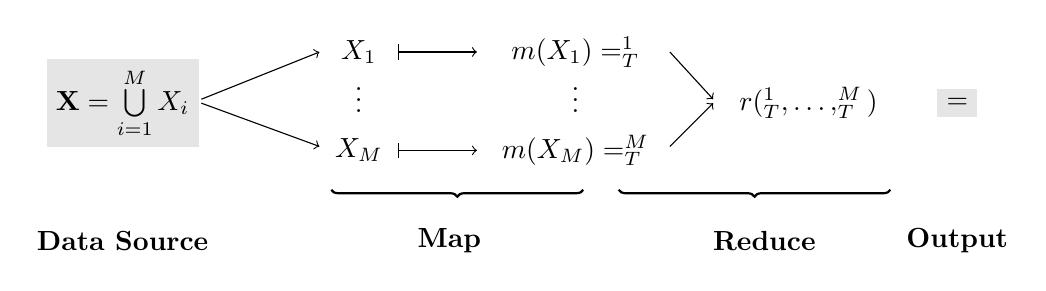
\begin{tikzpicture}
      \draw (-2.5,0.35) node[rectangle,fill=black!10] { $\mathbf{X} = \bigcup\limits_{i=1}^M X_i$ };
      \draw (-2.5,-1.4) node {\textbf{Data Source}};

      \draw[->] (-1.5,0.4) -- (0,1);
      \draw[->] (-1.5,0.35) -- (0,-0.2);

      \draw (0.5,1) node[rectangle] {$X_1$};
      \draw (0.5,-0.25) node[rectangle] {$X_M$};

      \draw (0.5,0.5) node {$\vdots$};


      \draw[|->] (1,1) -- (2,1);
      %\draw (1.5,1.25) node {$m$};
      \draw (3.25,1) node {$m(X_1) = \barw_T^1$}; %X_1'

      \draw[|->] (1,-0.25) -- (2,-0.25);
      %\draw (1.5,0) node {$m$};
      \draw (3.25,-0.25) node {$m(X_M) = \barw_T^M$}; %X_M'

      \draw (3.25,0.5) node {$\vdots$};

      %\draw (2,-0.25) node[rectangle,draw=black] {$m(X_M)$};

      \draw[->] (4.45,1) -- (5,0.4);
      \draw[->] (4.45,-0.2) -- (5,0.35);

      %\draw (6.21,0.35) node {$r(X_1',\ldots,X_M')$};
      \draw (6.21,0.35) node {$r(\barw_T^1,\ldots,\barw_T^M)$};

      \draw[decorate,decoration={brace, mirror},thick] (0.15,-0.75) -- (3.35,-0.75); % node at (6.5,-.5) {}; 
      \draw (1.65,-1.4) node {\textbf{Map}};

      \draw[decorate,decoration={brace, mirror},thick] (3.8,-0.75) -- (7.25,-0.75); % node at (6.5,-.5) {}; 
      \draw (5.65,-1.4) node {\textbf{Reduce}};

      \draw (8.1,0.35) node[rectangle,fill=black!10] {$=\barbarw$}; %$\ \overline{w}$.
      \draw (8.1,-1.4) node {\textbf{Output}};

    \end{tikzpicture}
